%--------------------------------------
%	Chapter 4. ML Hit-Pair Predictor
%--------------------------------------


\doublespacing
\newpage
%\setcounter{section}{3}
%\section{The Compressed Pattern Space}
\chapter{Machine Learning Hit-Pair Predictor} 
\label{chapter-4}

In order to build a graph network to be used for track reconstruction, one must first consider the ability to identify compatible edge connections for seed building. A beneficial step towards enhancing this process is to reduce the number of fake seeds constructed and hence increase the accuracy in predicting such compatible hit-pairs. Future upgrades to particle detectors, will be particularly problematic for the silicon tracking detectors where hit occupancy is the largest. Therefore, it is essential that resource use is also reduced, whilst maintaining the capability to reconstruct tracks with minimal efficiency loss.

This chapter presents a methodology to accomplish such a task and is implemented in the optimisation of the HLT ID track seeding [X] software for ATLAS Run-3 and beyond. Section \ref{measurement-to-track-association} presents the development of an ML-based algorithm to predict if a pair of hits belong to the same track given input hit features, focusing on cluster width and inverse track inclination. The implementation of the trained predictor in the form of Look-Up Tables is presented in Section \ref{application-of-hit-pair-predictor}, alongside performance results including tracking efficiency and speed-up factor using simulated data is also discussed. \textbf{Work presented in XX conference.}


\section{Measurement to track association}
\label{measurement-to-track-association}

\subsection{Data Exploration and Feature Extraction}

%  Top quark simulation is often used for algorithm validation due of many possible final states including electron muon and $\tau$ lepton, \textit{b, c} and up quark.

- also write about fake seeds here
  - pixel only seeds, reducing the fake rate. 
% mention the importance of why pixel based ML-based classifier is needed, the hit occupancy etc - most advantageous and beneficial here.
%The training is focused on pixel-detector layers, being closest to the beamline and thereby an advantageous region to reduce the proportion of fakes. The classifier predictions are used as input in the Fast Tracking algorithm.

Seeds constructed at the combinatorial stage of ATLAS track seeding from the Run-2 geometry were used to extract hit-pairs to form a training dataset. Monte Carlo (MC) $t\bar{t}$ samples with centre-of-mass energy $\sqrt{s}$ = 13 TeV at mean pile-up interaction multiplicity $< \mu >$ = 80 were used. An illustration of a seed in the ID pixel layers is shown in Figure \ref{fig:triplet-illustration}. From each triplet seed, the inner doublet (defined as hit-pair 1 and 2) and outer doublet (defined as hit-pair 2 and 3) are extracted. For each doublet the minimum and maximum absolute inverse slope of the track, $|cot(\theta)|$, were calculated using $r$-$z$ coordinates and used as an input feature for training. $\theta$ is the angle of inclination of a hit-pair with respect to the $z$ axis. The longitudinal pixel cluster width, $w_{\eta}$, measured in the $\eta$ direction was also extracted, where $\eta$ is defined in Eq. \ref{eq:pseudorap}. The MC generated data in the [$|cot(\theta)|$, $w_{\eta}$ ] phase space behaves as a set of 1-dimensional distributions, each with discrete $w_{\eta}$. This characteristic is exploited to form an ensemble of predictors. MC truth for seeds and their corresponding doublets were extracted from ATLAS track seeding and used as targets in training. Doublets with correct hit association were defined as truth 1, for which its hit-pairs belong to the same track. Conversely doublets with incorrect hit association defined as truth 0, for which its hit-pairs do not belong to the same track. Hit-pairs for the pixel barrel and endcap are handled separately in order to build regional classifiers, where a similar methodology was used for both outlined in Section ...


\begin{figure}[!htbp]
\centering
    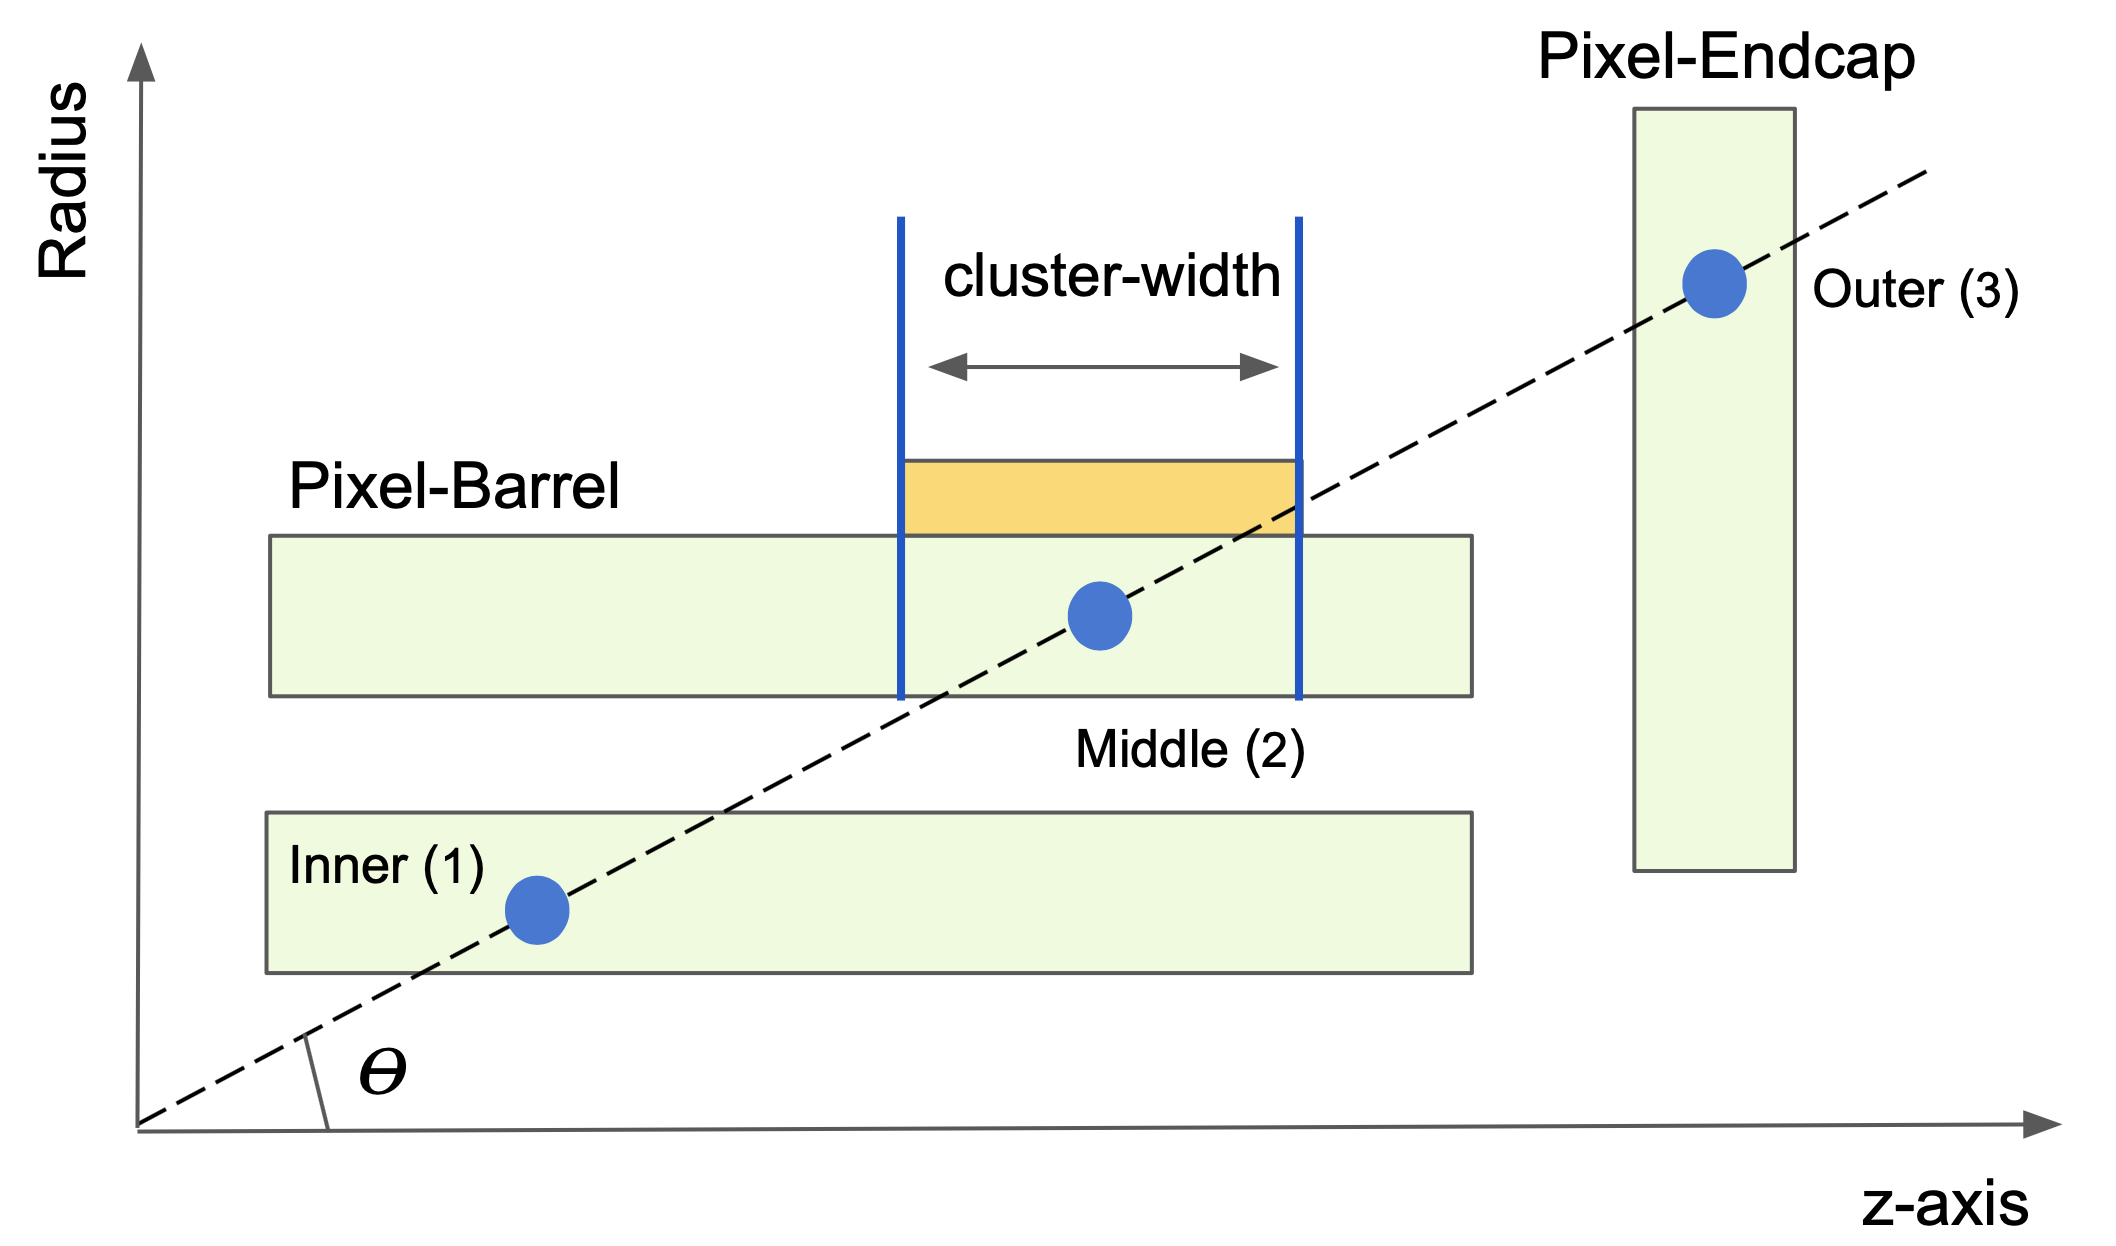
\includegraphics[width=0.8\linewidth]{images/4-ml-based-predictor/triplet_illustation.png}
    \caption{Seed illustration in the $r$-$z$ plane (mm) of the ID. The inner doublet consists of hits 1 and 2 and the outer doublet consists of hits 2 and 3. The longitudinal pixel-cluster width $w_{\eta}$ (mm) is measured in the direction of $\eta$, where $\theta$ is the angle of inclination with respect to the $z$ axis.}
\label{fig:triplet-illustration}
\end{figure}


\subsection{Classifier Development}

\subsubsection{Not-so-Naive Bayes}

The basis of Bayes’ theorem \cite{naive-bayes} is used to build a classifier to discriminate between doublet classes, for both the barrel and endcap regions. Bayesian analysis is based on having a prior probability of belief of an outcome of an event and a likelihood probability, where naive Bayes’ assumes that the conditional probabilities of the independent variables are statistically independent. The final classification is produced by computing the posterior probability by combining both the prior beliefs and the likelihood, which then determines the most probable class label. Using Bayes’ theorem is advantageous in this data-driven setting, as prior knowledge of the behaviour of the system is known. The posterior probability $P(c|x)$ that a given data point x belongs to class c is defined as:

\begin{equation} \label{naive-bayes}
    P(c|x) = \frac{P(x|c)P(c)}{P(x)}
\end{equation}

$P(x|c)$ is the conditional likelihood, $P(c)$ is the class prior probability and $P(x)$ is the predictor prior probability, used for normalisation and calculated from the number of data points belonging to class $c$.

Bayes' theorem is implemented using a generative model for each class. This was achieved by computing the likelihood function via a Kernel Density Estimate (KDE) for each of the 1-dimensional $\tau$ distributions, forming a set of generative Bayesian classifiers. This method removes the 'naive' element and performs the same classification with a more sophisticated generative model for each class.

\subsubsection{Kernel Density Estimation}

KDE is a non-parametric approach to estimate the probability density function of a random variable. The idea is that a kernel function is defined and centred on each data point in the sample. The sum of these functions together forms the kernel density estimate. The kernel density is defined as:
    
\begin{equation} \label{eq2}
    \hat{f}(x) = \frac{1}{Nh}  \sum_{i=1}^{N} K \left( \frac{x - x_i}{h} \right)
\end{equation}

where $K(x)$ is the kernel function, typically a smooth, symmetric and non-negative function, $h > 0$ is the smoothing bandwidth that controls the amount of smoothing applied to the function and N is the number of sample points used for normalisation \cite{kde}. The KDE must be normalised in order to represent a probability density. For this study the Gaussian kernel function is implemented to approximate the probability density at each data point in the sample. One advantage of using KDE is that it provides a more flexible estimator parameterised by $h$. The Gaussian kernel is defined as:
    
\begin{equation} \label{eq3}
    K(x) = \frac{1}{\sqrt{2\pi}} e^{\frac{-x^2}{2}}
\end{equation}

The choice of bandwidth is important, as increasing the bandwidth too high results in a smooth distribution where granular information is lost (over-smoothing). When using a bandwidth that is too small, this can lead to narrow peaks in close proximity to each other, resulting in a very noisy distribution (under-smoothing). There are several methods to determine the optimum bandwidth discussed in \cite{bandwidth-selection-methods}, many of which show similar properties. The method used in this study was the so-called \textit{Silverman's rule of thumb}, which works only for 1-dimensional data. Silverman's rule finds the bandwidth that minimizes the mean integrated squared error assuming that the data is Gaussian and a Gaussian kernel was used.

\subsection{Classifier Training}


\begin{figure}[!htbp]
\centering
    \begin{subfigure}[a]{0.86\textwidth}
        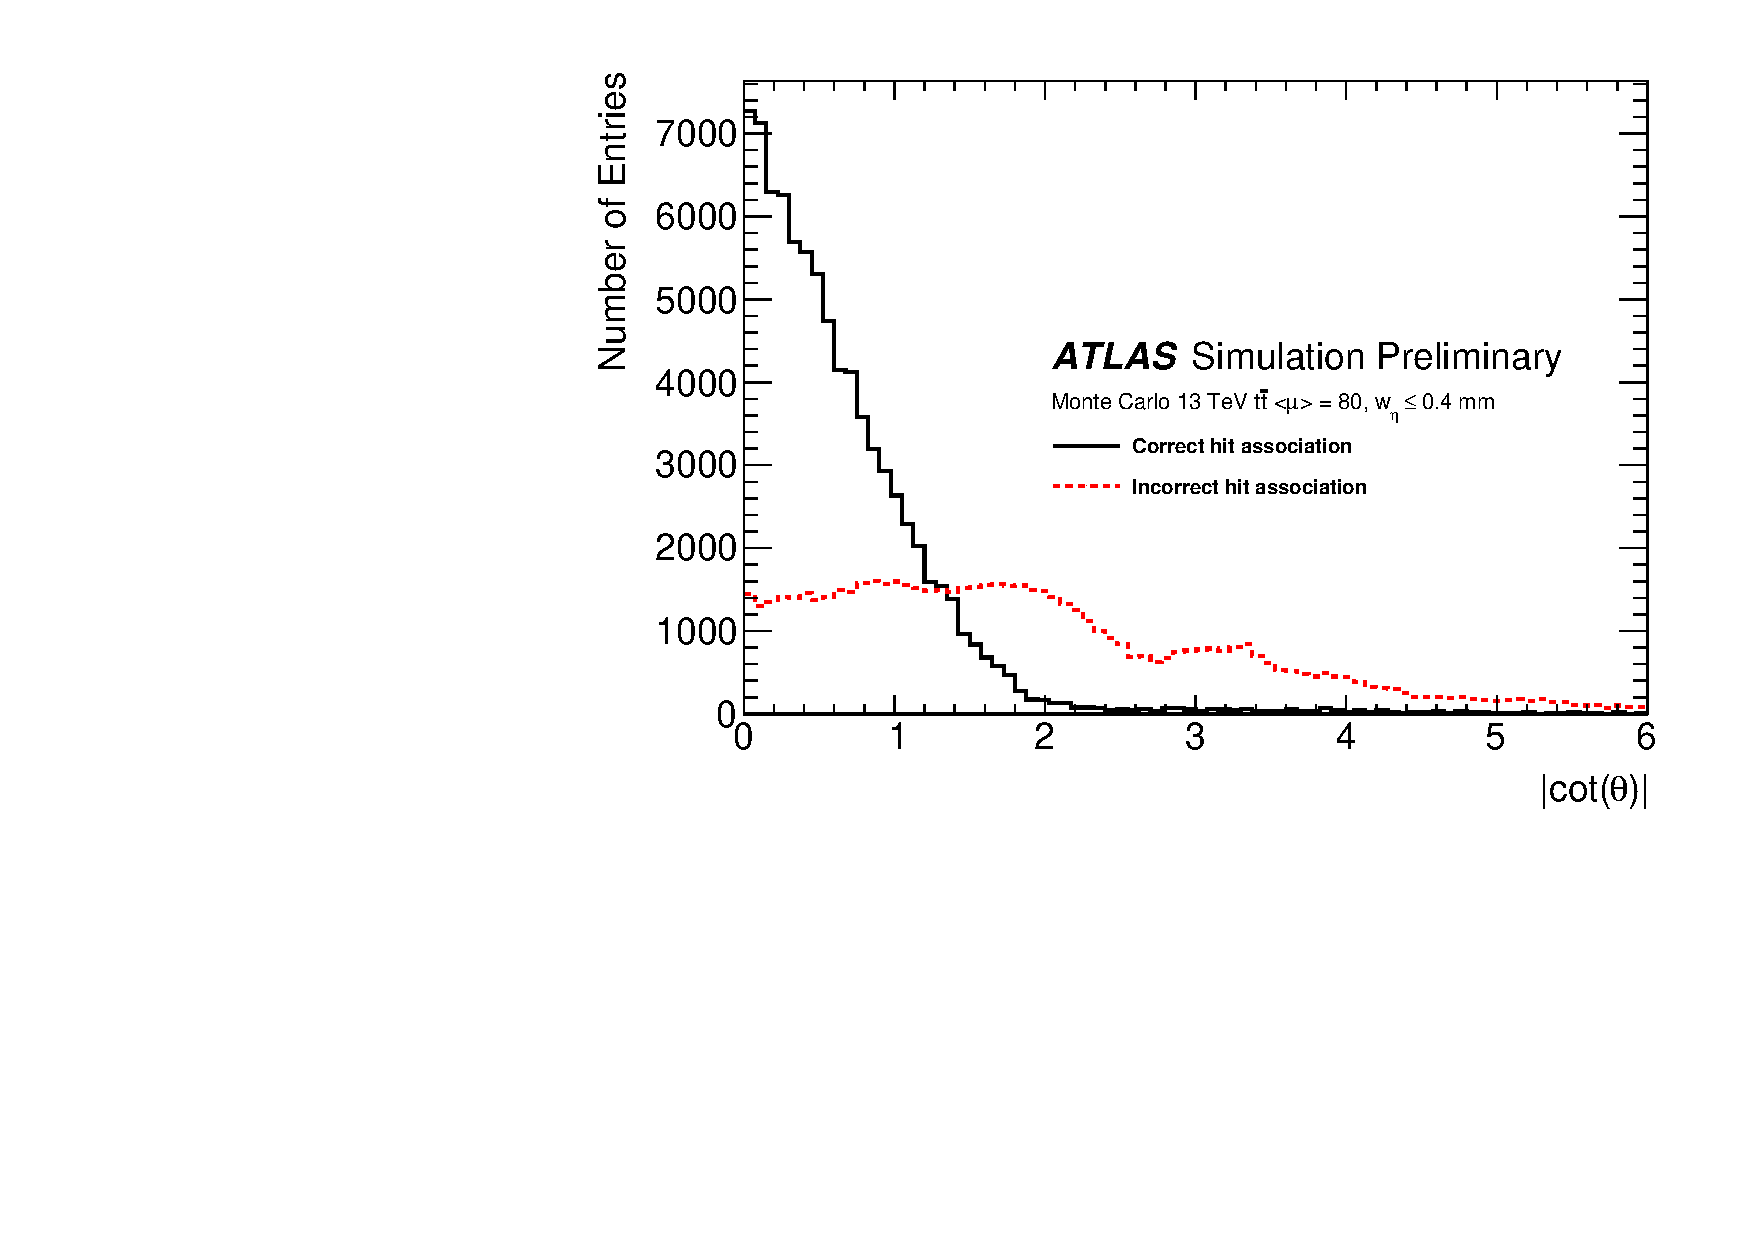
\includegraphics[width=\linewidth]{images/4-ml-based-predictor/histo.pdf}
        \caption{XXXX}
    \end{subfigure}
    \hfill
    \begin{subfigure}[b]{0.86\textwidth}
        \centering
        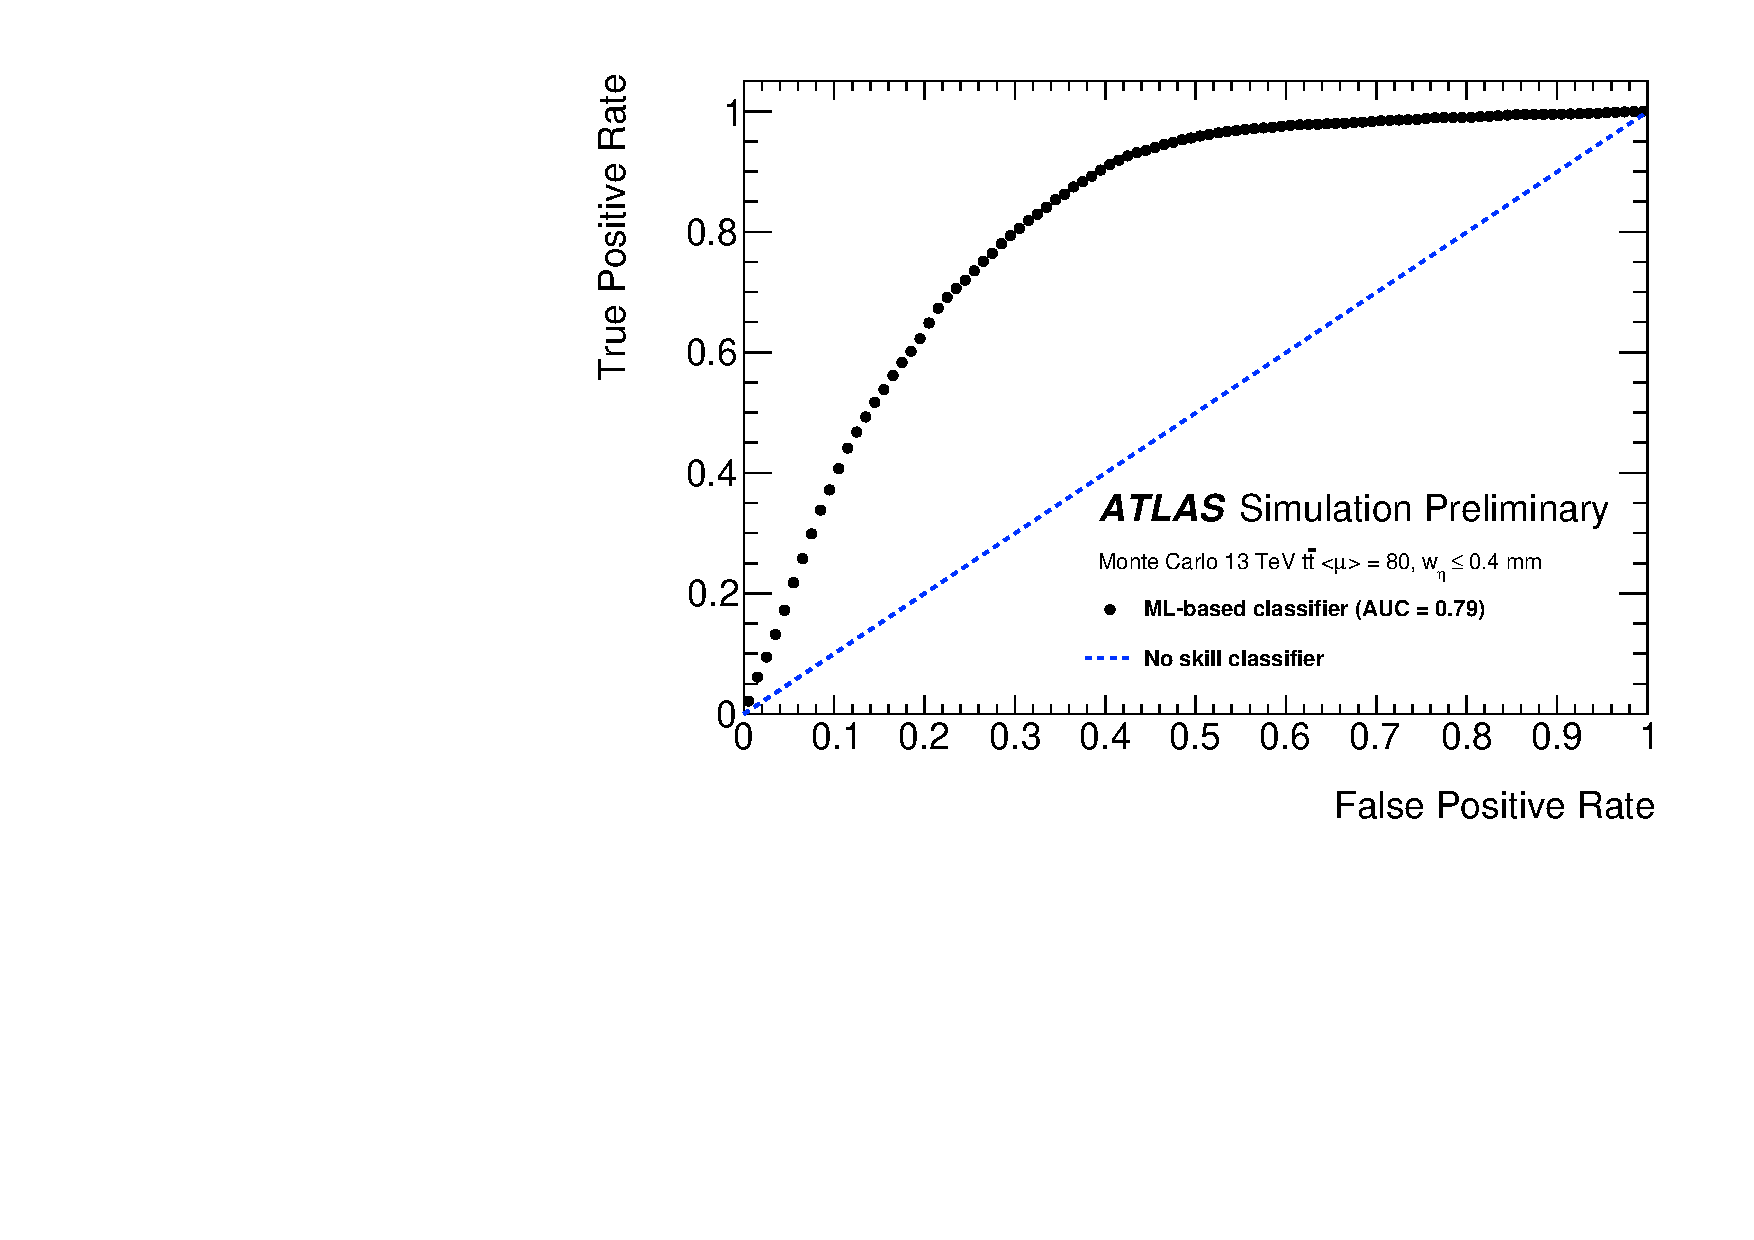
\includegraphics[width=\linewidth]{images/4-ml-based-predictor/roc.pdf}
        \caption{XXXX}
    \end{subfigure}
\caption{XXXX}
\label{fig:1-dimensional-classifier-training}
\end{figure}


\subsection{Probability Calibration}

\subsection{Classifier Predictions and Evaluation}

\begin{figure}[!htbp]
\centering
    \begin{subfigure}[a]{0.86\textwidth}
        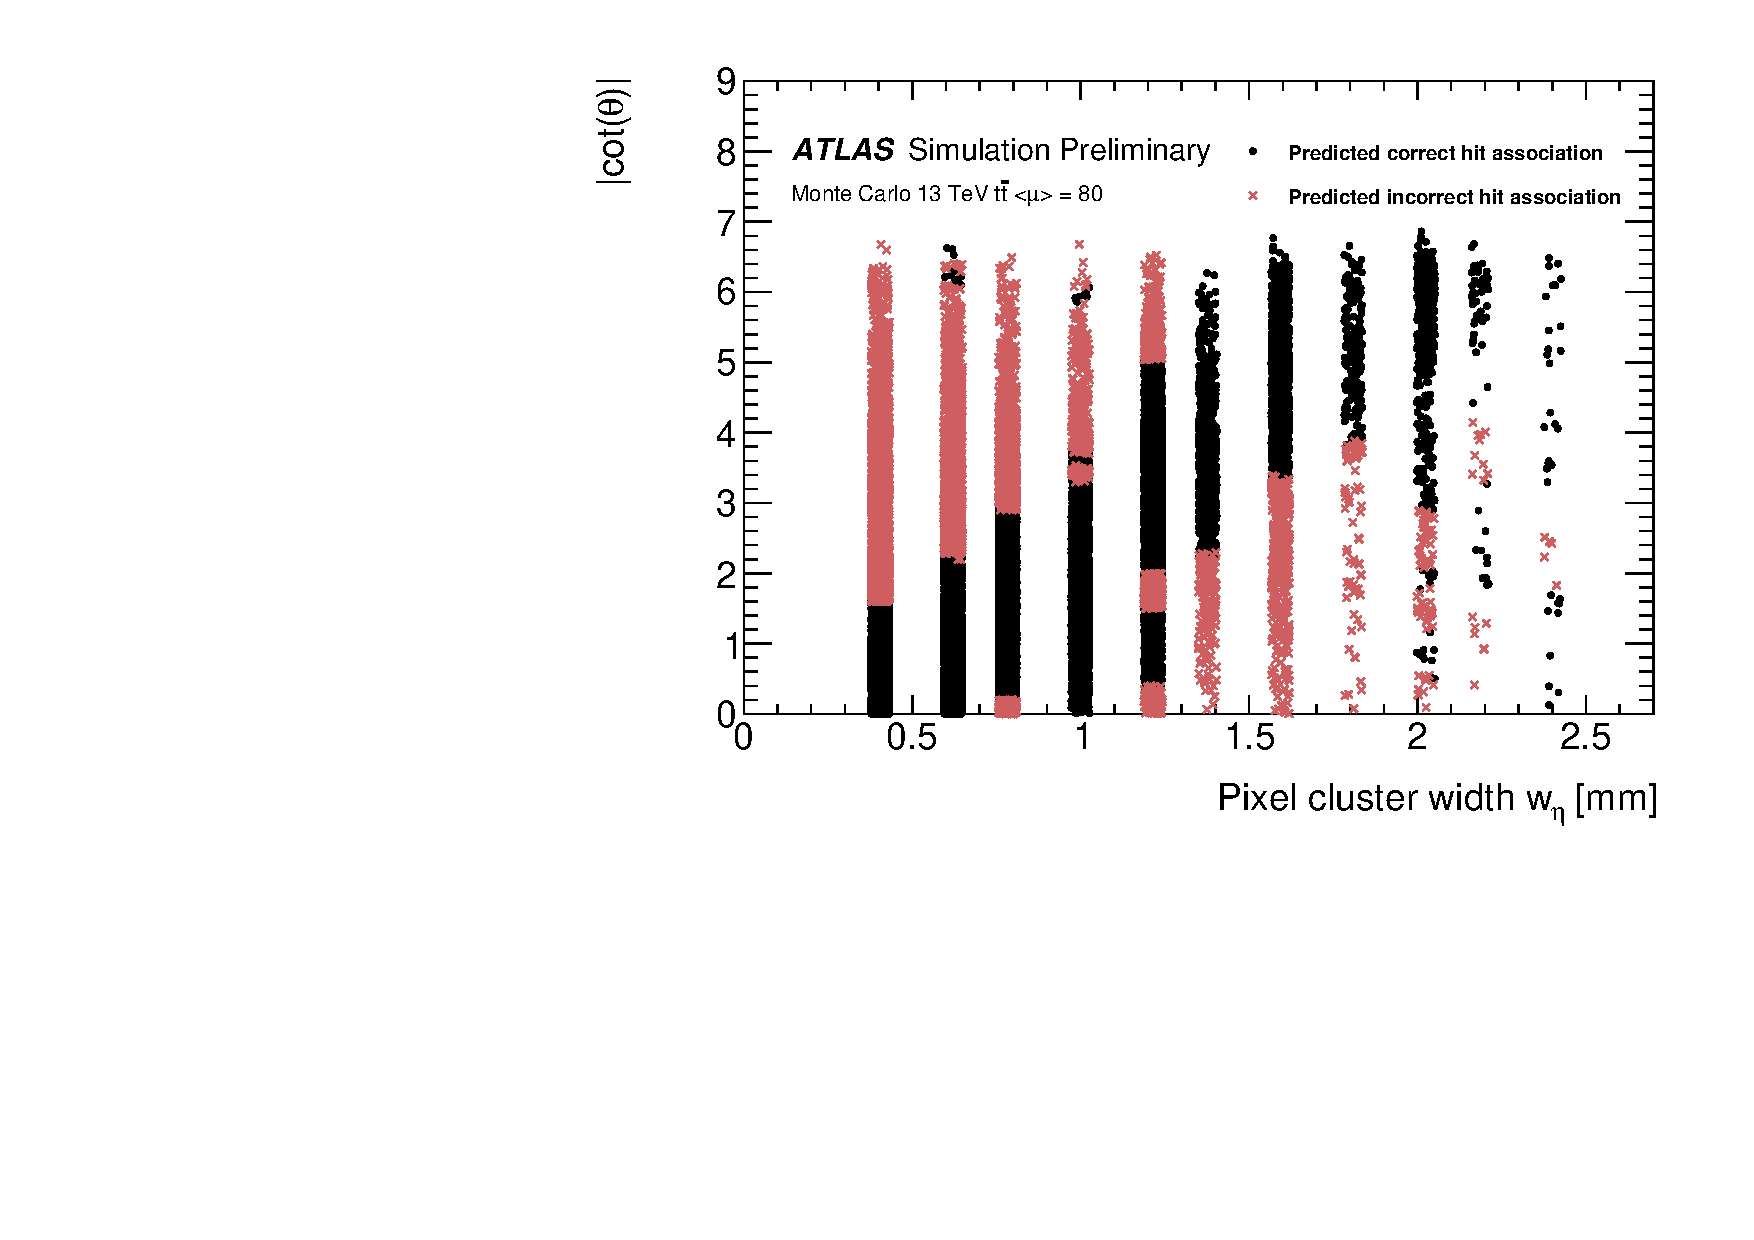
\includegraphics[width=\linewidth]{images/4-ml-based-predictor/scatter_kde_predictions.pdf}
        \caption{XXXX}
    \end{subfigure}
    \hfill
    \begin{subfigure}[b]{0.86\textwidth}
        \centering
        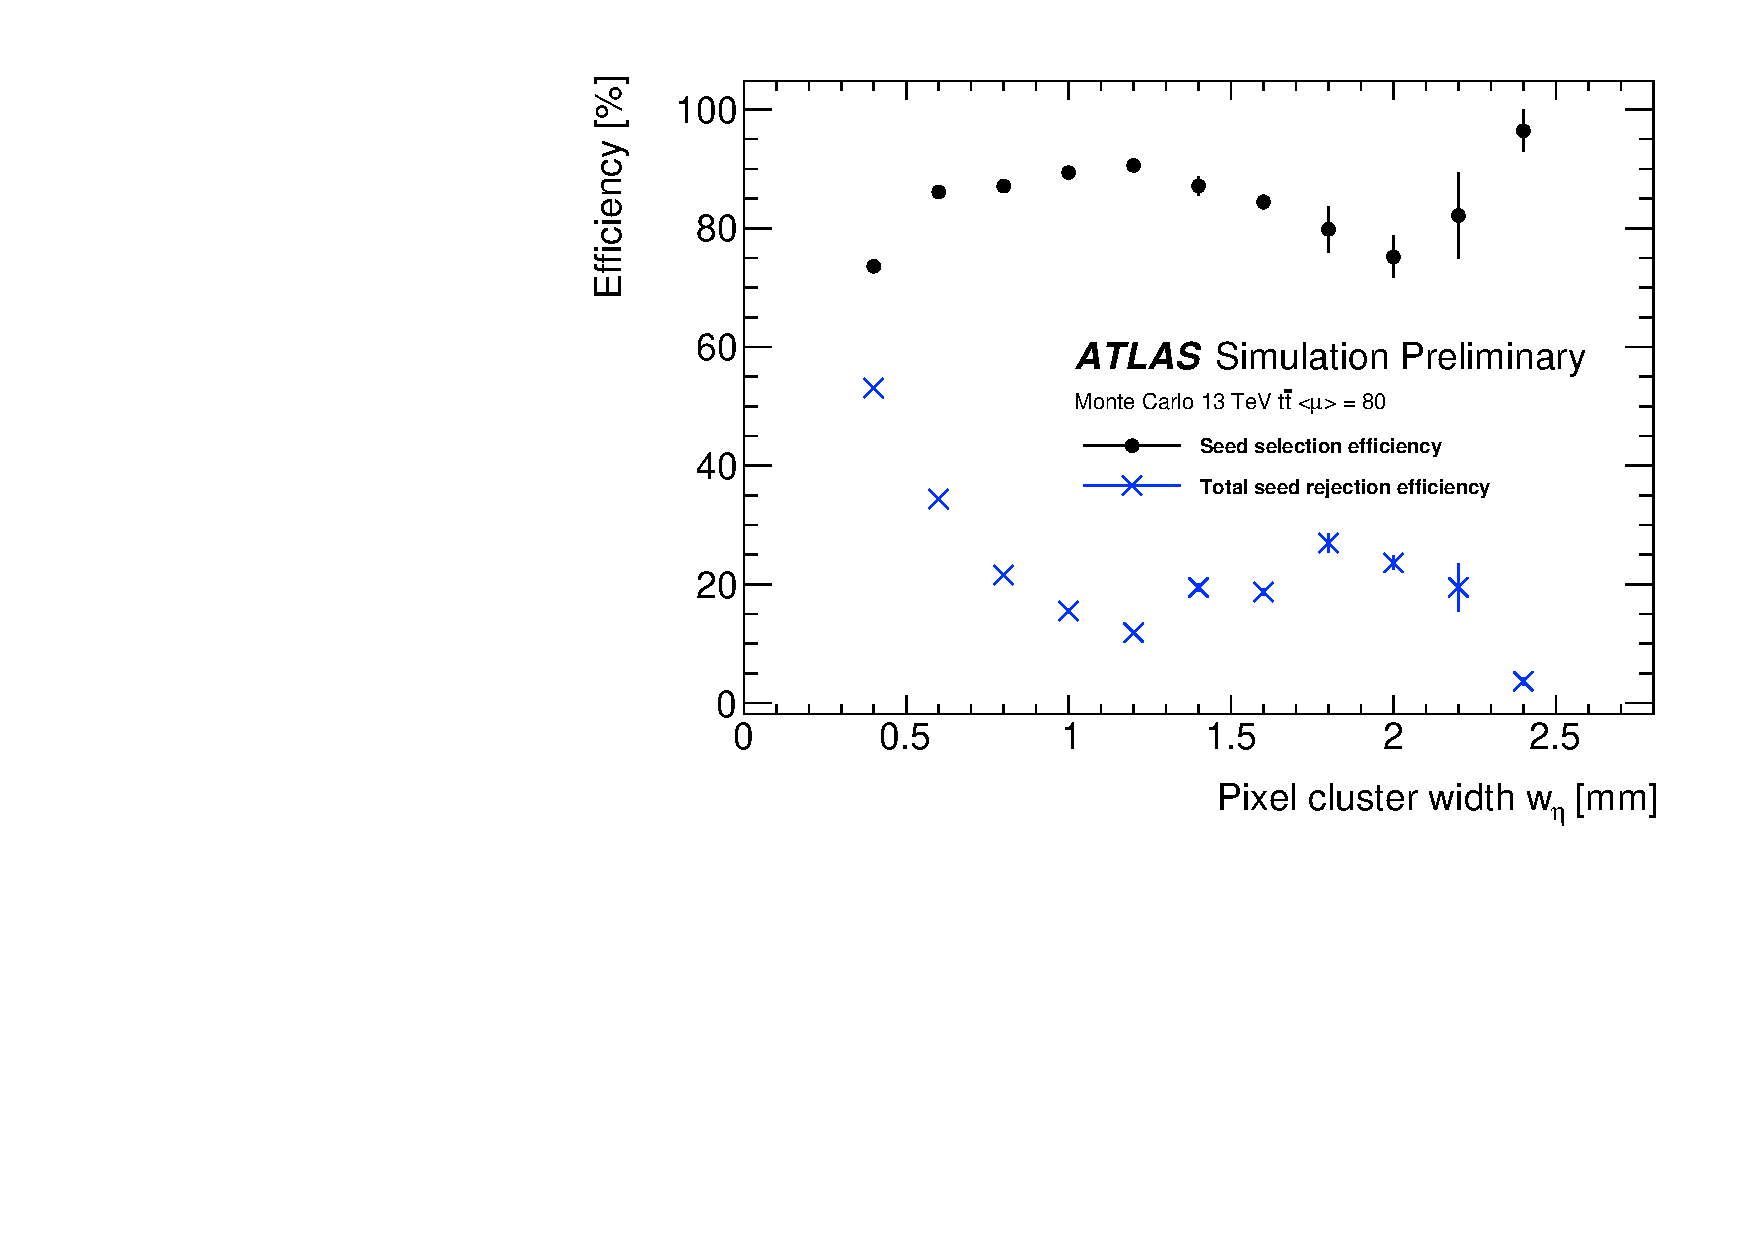
\includegraphics[width=\linewidth]{images/4-ml-based-predictor/triplet_eff_metrics.pdf}
        \caption{XXXX}
    \end{subfigure}
\caption{XXXX}
\label{fig:predictions-pixel-barrel-and-triplet-efficiencies}
\end{figure}


\section{Application of hit-pair predictor}
\label{application-of-hit-pair-predictor}

\subsection{Look-Up Table Generation}

Classifier predictions are converted into Look-Up Tables (LUT) such that the acceptance region can be fed into the FTF. Using a predefined LUT is a much more efficient procedure than computing class label on the fly and it is very low cost to store in memory. It consists of binning both the W eta axes (45 bins between 0.0 - 3.0) and the $\tau$ axes (30 bins between 0.0 - 3.0), recording the bin numbers to accept. These divisions were chosen such to compare with the current estimation, referred to as strict LUT.

\subsubsection{Morphological Filtering}

An ensemble approach was taken combining the strict LUT and KDE predictions. Morphological filtering was then applied to achieve a smoothed structure. Morphological filtering is an image processing technique whereby non-linear transformations are applied to the binary matrix of an image, altering the features. Such non-linear operations include dilation and erosion. Dilation enlarges bright regions and shrinks dark regions, whereas erosion does the inverse of this. A combination of dilation and erosion was applied to the ensemble LUT via rectangular structuring elements, in order to encourage horizontal
extrapolation of the acceptance region. The binned predictions from the KDE classifiers and smoothed LUTs are shown in Figures 9 and 10; orange representing acceptance regions and blue rejection regions.
Referring to 9a, KDE predictions for the barrel coincide well with the ’linear corridor’ estimation from the strict LUT. Whereas a V-shaped LUT is obtained for the endcap region.


\subsection{ML filtering modes}

\subsection{Seed Classes}



\subsection{Performance Evaluation}

There is little deviation from the standard trigger seeding with application of the machine learning extensions, where the average tracking efficiency achieved was 93.9\% and the greatest efficiency loss from the standard trigger seeding is at large $\lvert \eta \rvert$.

\begin{figure}[!htbp]
\centering
    \begin{subfigure}[a]{0.86\textwidth}
        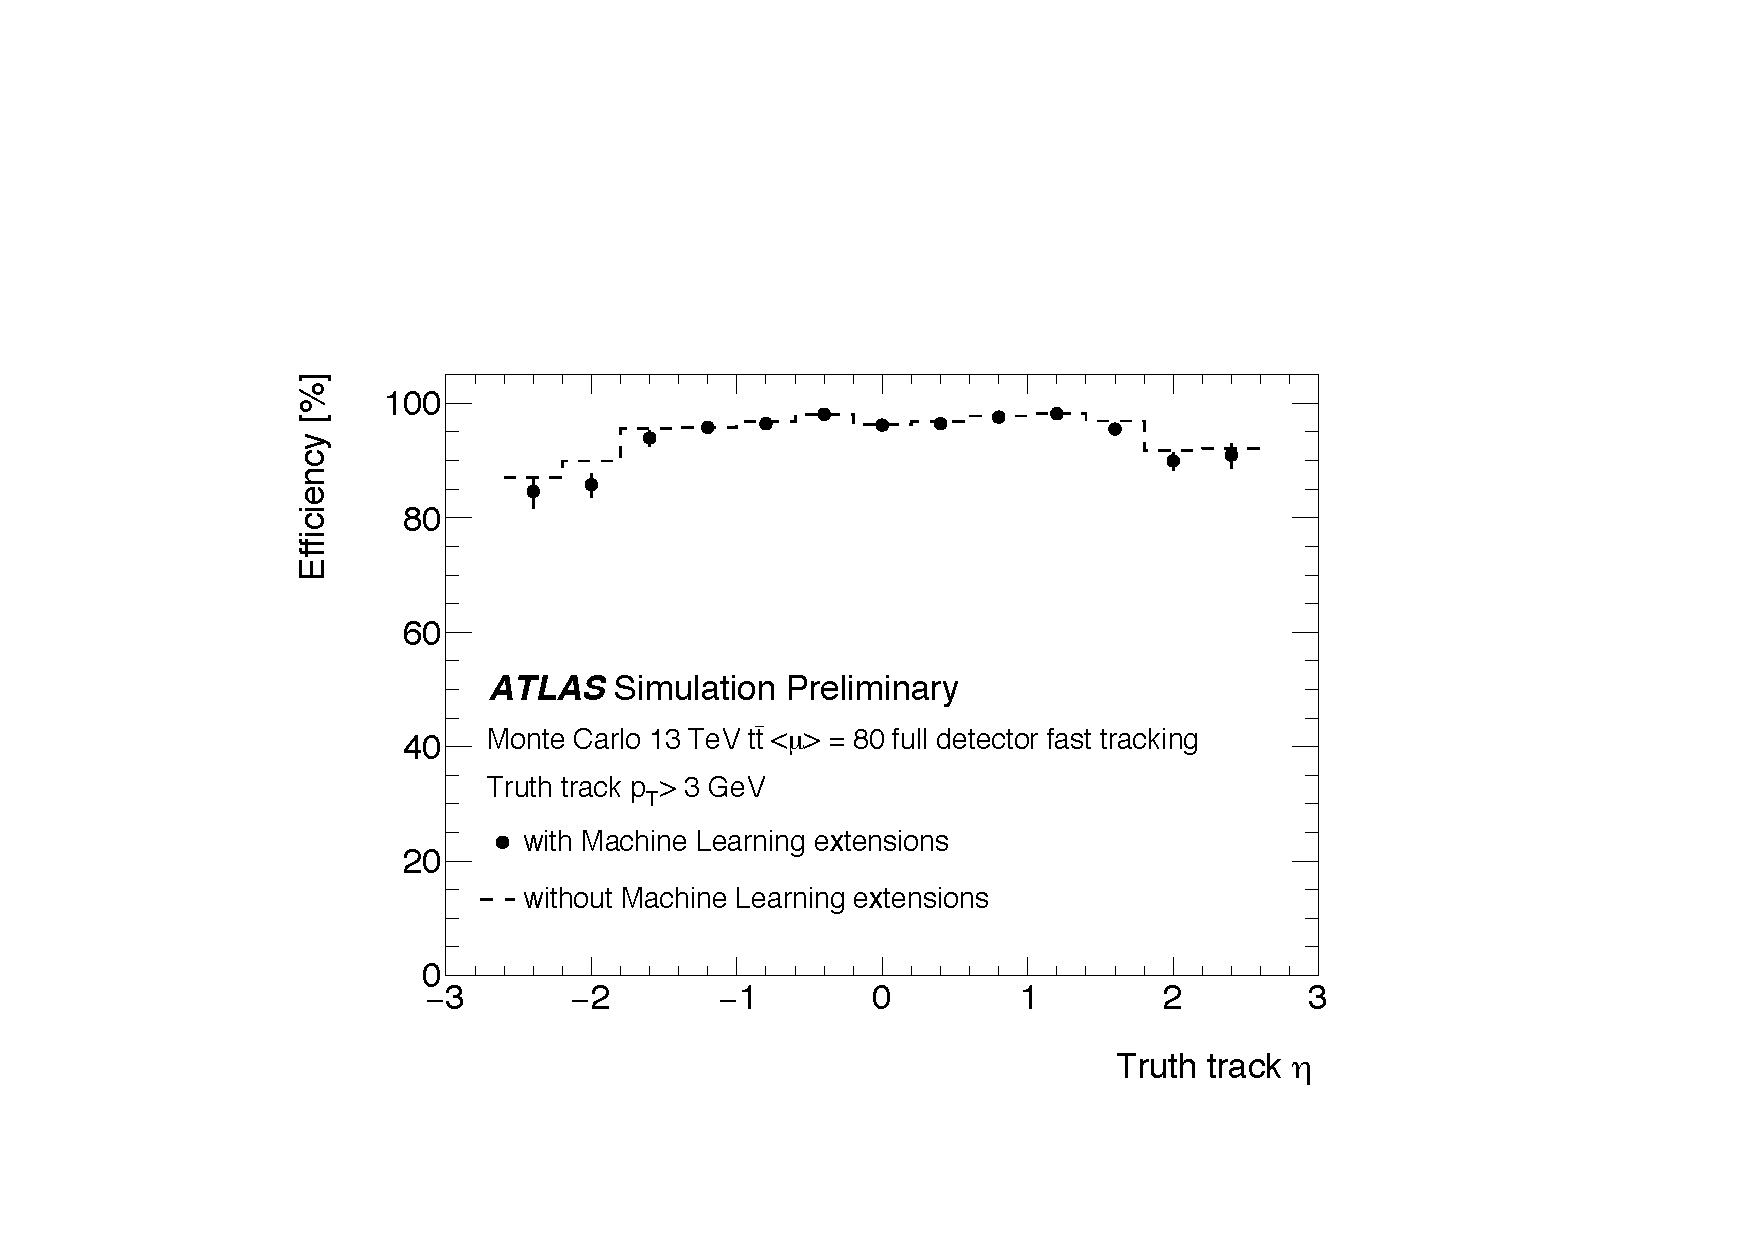
\includegraphics[width=\linewidth]{images/4-ml-based-predictor/efficiency_eta.pdf}
        \caption{Efficiency vs. MC truth track $\eta$}
    \end{subfigure}
    \hfill
    \begin{subfigure}[b]{0.86\textwidth}
        \centering
        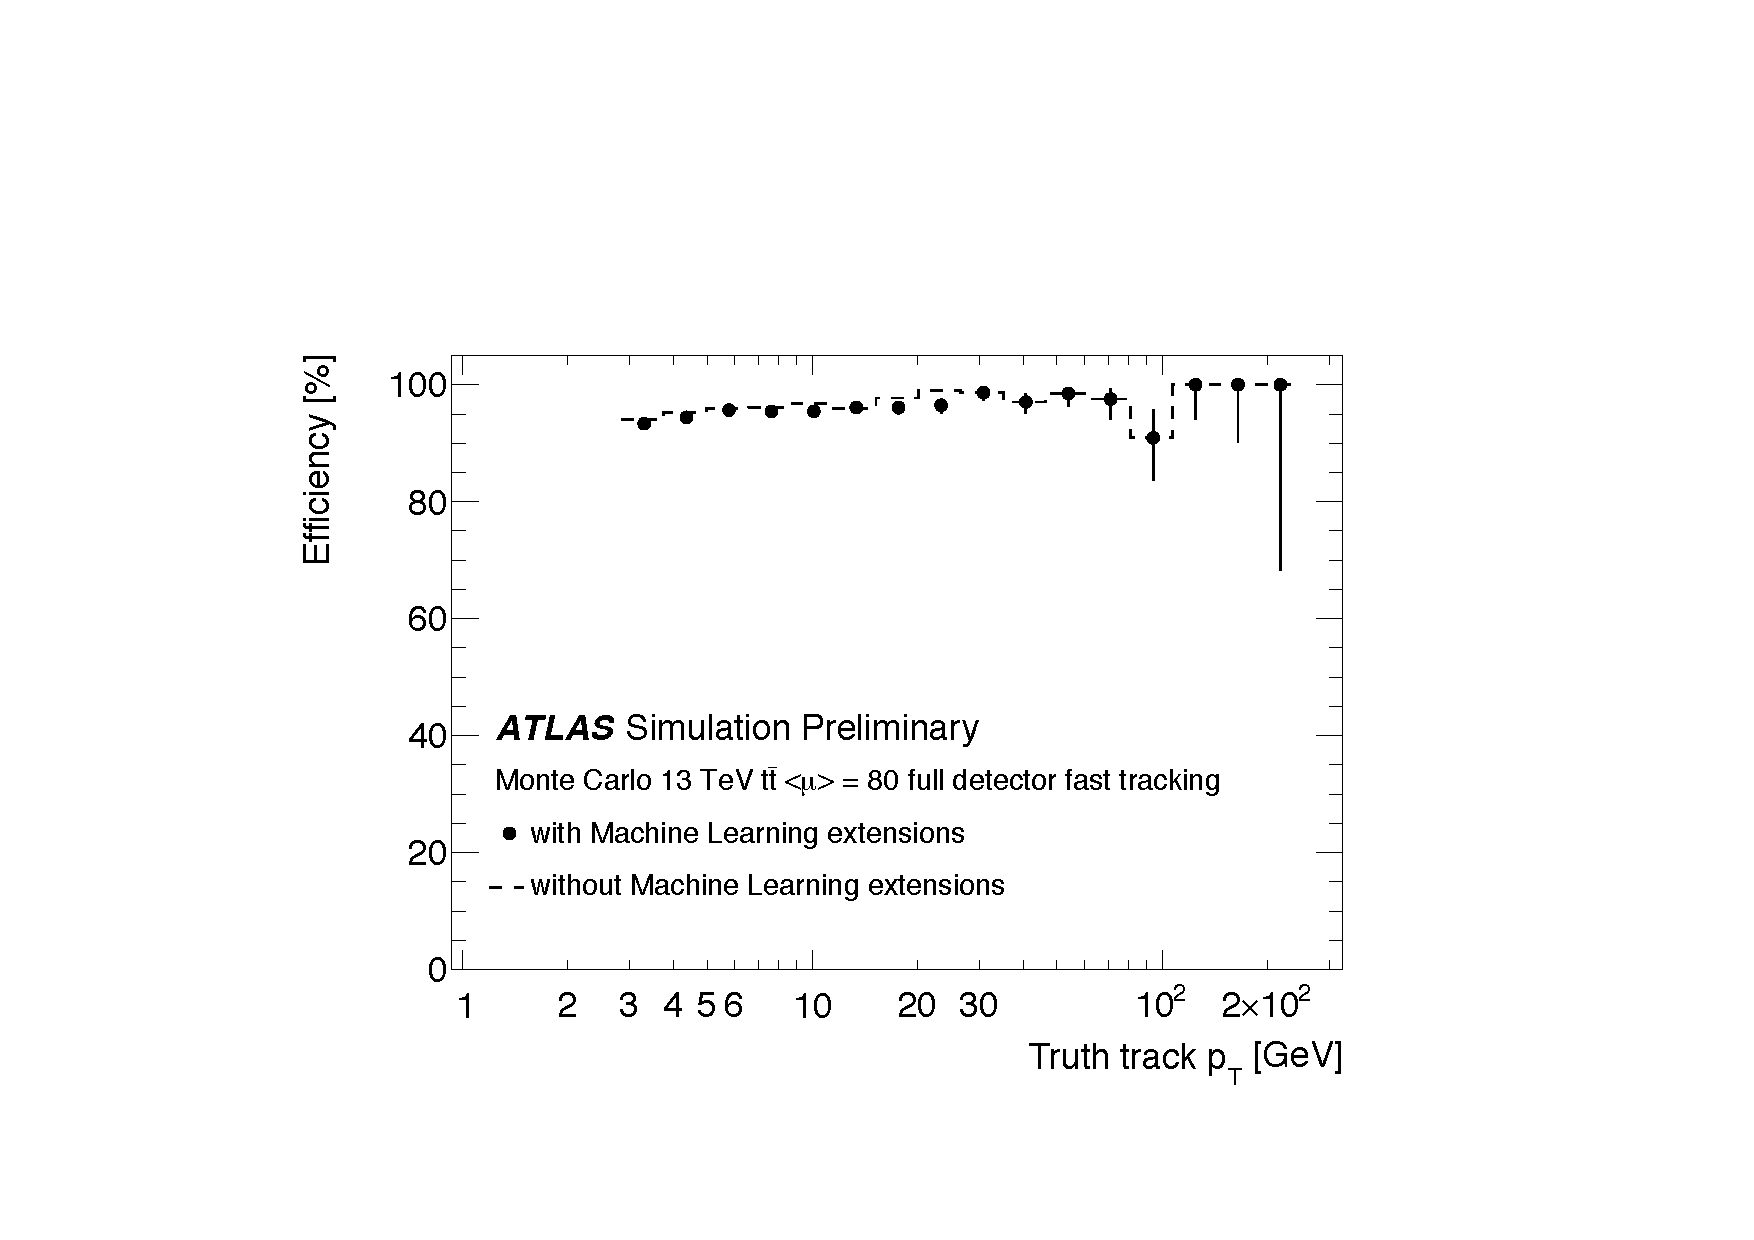
\includegraphics[width=\linewidth]{images/4-ml-based-predictor/efficiency_pT.pdf}
        \caption{Efficiency vs. MC truth track $p_{\mathrm{T}}$}
    \end{subfigure}
\caption{Tracking efficiencies as a function of track parameters, for $p_{T}$ > 3 GeV for the ATLAS full detector tracking with $t\overline{t}$ Monte Carlo 13 TeV and mean pile-up interaction multiplicity of $\langle \mu \rangle$ = 80. The data points show the efficiency when using machine learning extensions in the seed building stages of the fast tracking trigger in the ATLAS pixel detector, prior to the track fitting. The dashed line shows the efficiency of the standard trigger seeding with no application of machine learning extensions. The errors shown are purely statistical \cite{public-hlt}. }
\label{fig:efficiencies-ml-hit-pair-predictor}
\end{figure}



\subsubsection{CPU Time Comparison}

Table \ref{tab:cpu} summarises the breakdown in speed-up factor achieved at various stages within the \texttt{Fast Tracking} trigger algorithm, with the application of the trained LUT for the pixel region. The greatest saving in CPU time is achieved during the \texttt{Seed Processing} stage, as a direct result of a significant reduction in the number of seeds. The average number of seeds processed for a given region of interest for the standard tracking is $O(10^{4})$, whereas with the introduction of ML filtering for pixel seeds, about 78\% fewer seeds were observed. This significant reduction in CPU time does not only benefit the \texttt{Seed Processing} stage of the combinatoric track following, but also propagates to \texttt{Track Fitting}.

\begin{table}[htb!]
\caption{Performance of the ATLAS full detector tracking with MC 13 TeV $t\bar{t}$ samples at $<\mu> = 80$, with the application of ML extensions for filtering on pixel detector hit-pairs in the \texttt{Fast Tracking} trigger stage \cite{public-hlt}. The total speed-up factor and breakdown of speed-ups at different stages of the \texttt{Fast Tracking} trigger algorithm are presented, each speed-up is presented with respect to the standard trigger seeding where no ML extensions were applied.}
\begin{center}
\begin{tabular}{llll}
\toprule
Total Speed-up Factor & Seed Generation & Seed Processing & Track Fitting \\
\hline
2.3 & 1.3 & 3.3 & 1.5 \\ 
\bottomrule
\end{tabular}
\end{center}
\label{tab:cpu}
\end{table}

\subsubsection{Changing Pileup Conditions}
Table \ref{tab:pileup} summarises the relative efficiency loss and relative speed-up factor, with application of ML extensions for the ATLAS pixel detector in various mean pile-up interaction multiplicities $<\mu>$. The speed-up factor increases as $<\mu>$ increases with minimal loss in efficiency.

\begin{table}[htb!]
\caption{Performance of the ATLAS full detector tracking with MC 13 TeV $t\bar{t}$ samples at $<\mu>$ = 40, 60 and 80, with the application of ML extensions for filtering on pixel detector hit-pairs in the \texttt{Fast Tracking} trigger stage prior to the track fitting \cite{public-hlt}. The absolute loss in average tracking efficiency and the total speed-up factor for seeded track finding in the ATLAS pixel detector are presented with respect to the standard trigger seeding where no ML extensions were applied. The efficiency loss is mainly observed at large $|\eta|$. The statistical uncertainties in efficiencies are $O(10^{-3})$, hence are not quoted.}
\begin{center}
\begin{tabular}{ccc}
\toprule
$<\mu>$ & Efficiency Loss (\%) & Total Speed-up Factor  \\
\hline
40 & 0.7 & 1.6 \\
60 & 0.7 & 2.1 \\
80 & 1.1 & 2.3 \\
\bottomrule
\end{tabular}
\end{center}
\label{tab:pileup}
\end{table}


\section{Other Approaches}
\subsection{Multiple Acceptance Regions}

When training With varying permutations of train and test sets, a second acceptance region was frequently predicted for the barrel at low-cluster width and high track inclination angle, highlighted in Figure \ref{fig: multiple-acceptance}. The spacepoints predicted as belonging to the $good$ doublet class at the tail ends of these distributions were isolated and their local cluster position in the $\eta$ direction were considered, see Figure \ref{fig: multiple-acceptance}. The majority of hits possessed the largest absolute local cluster position. This was observed for each occurrence of a second acceptance region appearing at low cluster-width and high track inclination. This corresponds to the extremes of the barrel module, since its dimensions are approximately $20mm$ $x$ $60mm$ \cite{pixel-module-dimensions}, and hence the second acceptance region had originated from module edge pixels. These spacepoints would need to be dealt with separately or accepted by default. One reason for this is, due to the fact that the morphological smoothing is applied uniformly to an image, this will affect the shape of the main acceptance region for the barrel and will introduce a greater proportion of fakes by dilation.
    

\subsection{Support Vector Machine}

% See this website for further explanation 
% https://towardsdatascience.com/support-vector-machine-introduction-to-machine-learning-algorithms-934a444fca47

% multi class classification: one-to-rest
% https://towardsdatascience.com/multiclass-classification-with-support-vector-machines-svm-kernel-trick-kernel-functions-f9d5377d6f02

Another supervised learning algorithm investigated was the Support Vector Machine (SVM) \cite{svm}. The objective of the SVM classifier is to find a hyperplane (known as a decision boundary) in a N-dimensional space (where N is the number of features) that distinctly classifies the data points and is typically used in binary classification. The optimal decision boundary is one which maximizes the margins between both classes, this provides some reinforcement that future data points can be classified with more confidence. For non-linear decision boundaries, the SVM uses the so-called \textit{kernel trick} to project the data into a higher dimensional space. 


A prior step to training the SVM classifier, was to apply Principal Component Analysis (PCA).

A combination of Principal Component Analysis (PCA) and SVM was applied. PCA is commonly used as a dimensionality reduction technique \cite{pca}, however in this instance it is applied to remove the ordinal nature (the discrete bands) which affects the SVM and hence obtain a continuous 2D-dimensional phase space. 
    
A hyper-parameter sweep of different kernels was executed using cross-validation and the polynomial kernel of degree 3 was found to produce the highest TPR. The predictions of PCA-SVM on the barrel data is shown in Figure \ref{fig:barrel-svm-pca}, the red (orange) region shows which doublets are accepted and the blue region shows which doublets are rejected. The corresponding data points also reflect class predictions. 

SVMs generally perform well, even when trained with imbalanced data sets. This coupled with the fact that a distinct decision boundary could be easily extracted and converted into a LUT would lead to less ambiguity in comparison to applying an extrapolation using morphological smoothing. However, there are key disadvantages by using a SVM classifier rather than Bayes' theorem in this instance. The probabilistic information contained within each discrete 1 dimensional distribution of $w_{\eta}$ is lost, which is an important feature when tuning each individual distribution. Additionally, the SVM typically fits a continuous function for the decision boundary and hence may not be strict enough in certain regions. This factor is important when considering the number of fake seeds being accepted using a LUT generated from such a decision boundary. 


\begin{figure}[!htbp]
\centering
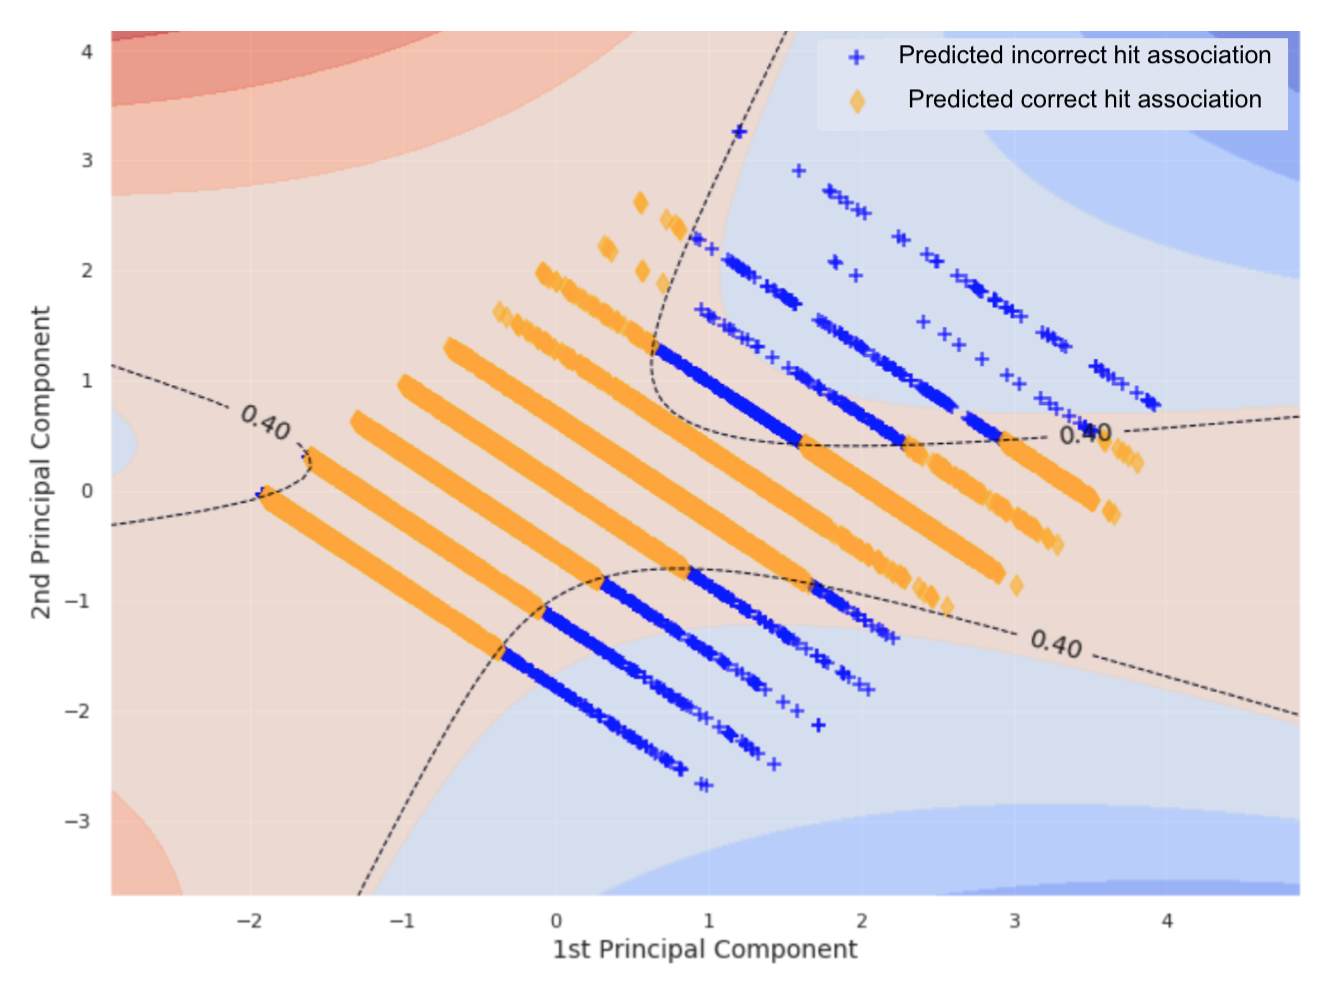
\includegraphics[width=0.85\linewidth]{images/4-ml-based-predictor/barrel-svm-pca.png}
\caption{PCA transform applied to the pixel barrel hit pairs. SVM classifier decision boundary predictions are shown in the above plot. The black dotted line represents the threshold value of 0.40, yielding a TPR of 95\%. The SVM kernel used for the classifier was a polynomial degree 3 kernel with hyperparameters $C=0.75$ and $\gamma=0.05$. 1st principal component indicates the axis of largest variance within the class with correct hit association doublet class.}
\label{fig:barrel-svm-pca}
\end{figure}

Figure \ref{fig:barrel-svm-pca} it is clear to see that the area of acceptance predicted by the SVM is much greater than the KDE based classifier. The seed multiplicity in these areas would inevitably lead to a larger amounts of time spent on processing seeds through the combinatorial stage of the FTF. Therefore this method was not pursued. However, a further investigation would be needed to evaluate the efficiency and speed-up provided from these predictions, compared with the KDE based classifier.


\subsection{Comparison with Deep Learning Algorithm}

Comparison with outrunner algorithm (number 2 in TrackML) - deep learning methodoloy vs. our classic ML approach.


\section{Conclusions}

% ---------------------------------------
% TODO
% ---------------------------------------
%At the end of this chapter, mention that a similar classifier was implemented to find pairs of hits for TrackML algorithm as well. Interestingly it also goes to a LUT input because this is the fastest way to do inference and implement this in any realistic detector setup, instead of training the classifier each time on the fly. Of course, for different geometrical setups or for particular signatures i.e. jets, the training would need to be done again specifically for that purpose.

As the luminosity, and hence collision rate, increases during future upgrades of the LHC program, novel and precise tracking methodologies, as well as efficient use of computing power will become an increasingly
important factor in the selection of physics objects.

The application of a ML-based classifier for seed selection in the ATLAS ID has provided significant CPU savings on trained MC data at various pileup levels. The trained predictor in the form of a LUT yields 2.3$\times$ speed-up with minimal loss in efficiency (1.1\%) at $< \mu >$= 80 compared with the standard trigger tracking. The developed ML pipeline provides a way to generate custom LUTs by training the predictor to yield a required TPR, dependent on the degree of efficiency required. Reducing the proportion of fakes at an earlier stage in the ATLAS HLT track seeding, ensures the reduction in CPU usage overall. Efficient use of computing power will become an increasingly important factor in the selection of physics objects as the luminosity and pileup increase during future upgrades of the LHC program.

%It is encouraging to see that the use of a ML based classifier for seed filtering in the ID, together with the proper selection of seed types, has provided significant CPU savings based on trained MC data. The application of the trained KDE based predictor in the form of a smoothed LUT for seed filtering within the barrel and endcap, as well as propagation of high purity seed types, yields greater than 2x speed up with minimal loss in efficiency, compared with the default. By applying an ensemble approach in LUT generation, this results in a much smaller drop in efficiency than using the strict LUT estimation alone. The use of different ML filtering modes applied to the triplets, can produce varying efficiencies (and speed up), where the three least redundant combinations are presented in this study. This procedure also shows greater efficiency across full range in η for the ID, compared with the strict LUT, which rejects a larger proportion of good seeds, particularly within the high seed multiplicity (low cluster width) range. Additionally, proper training and tuning of the classifier can yield a required TPR, therefore allowing the flexibility in strictness. By reducing the proportion of fakes an at earlier stage in the HLT track seeding, this ensures the reduction of bad seed propagation into later tracking stages and hence saving CPU.

